\section{Exécution \& tests} % (fold)
\label{sec:execution}

Pour ce projet, nous avons effectué des tests de validation sur quelques fonctions, afin de s'assurer que celles-ci marchaient correctement, et pouvoir plus facilement isoler les problèmes. 
De même, le code a été segmenté pour permettre une lecture plus aisée de l'ordre dans lequel s'effectuent les diverses opérations.

\section{Performances} % (fold)
\label{sec:perf}

Les courbes de performances ont été tracées avec gnuplot sur la version \og jouet \fg. Tous les temps sont en microsecondes.

\begin{figure}[H]
\centering
\lstinputlisting{comp_chinois_vol.conf}
\caption{Fichier de configuration utilisé pour les tests}
\label{fig:conf}
\end{figure}
Nous avons utilisé le fichier de configuration de la figure \ref{fig:conf} pour les tests. Ainsi, les grosses tâches étaient situées au début de la distribution linéaire et les premiers processus se voyait submergés de 10 grosses tâches durant 5e+5 $\mu s$. Pour changer de méthode (vol de tâche, restes chinois, etc), nous changions juste l'un des trois premiers paramètres. 

Dans un premier temps, nous avons comparé la distribution linéaire (i.e le processus $i$ calcule les tâches d'indices $i \times q$ à $(i+1) \times q$, avec $q$ le nombre de tâches par processus) et la distribution des restes chinois, sans le vol de tâches (voir Fig. \ref{comp_chinois_lin}). Alors que la distribution linéaire n'est pas très efficace, la distribution des restes chinois permet de mieux répartir les taches coûteuses entre les processus, ces taches coûteuses étant contiguës dans le tableau d'attribution des tests (cela se retrouve dans le calcul des rayons, où les tâches avec un temps de calcul élevé sont dans la même région).\\

\begin{figure}[H]
\centering
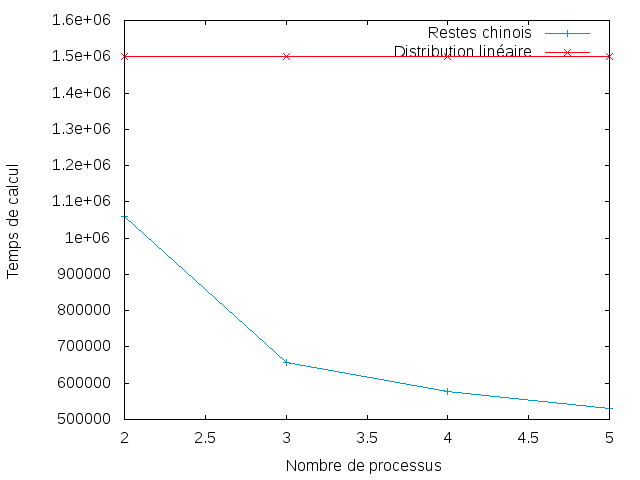
\includegraphics[width=0.8\textwidth]{comp_chinois_lin.png}
\caption{Pas de vol de tâche.}
\label{comp_chinois_lin}
\end{figure}

Dans un second temps, nous avons observé les performances de la distribution linéaire avec le vol de tâches. Les performances sont meilleures que sur les deux précédents cas, car une fois qu'un processus n'a plus de travail, il va chercher à en obtenir auprès des autres processus. Cela permet d'équilibrer la charge de calcul, malgré une mauvaise distribution. Ainsi, la figure \ref{vol_lin_lin} nous montre à quel point le vol de tâches est intéressant pour une distribution linéaire.

\begin{figure}[H]
\centering
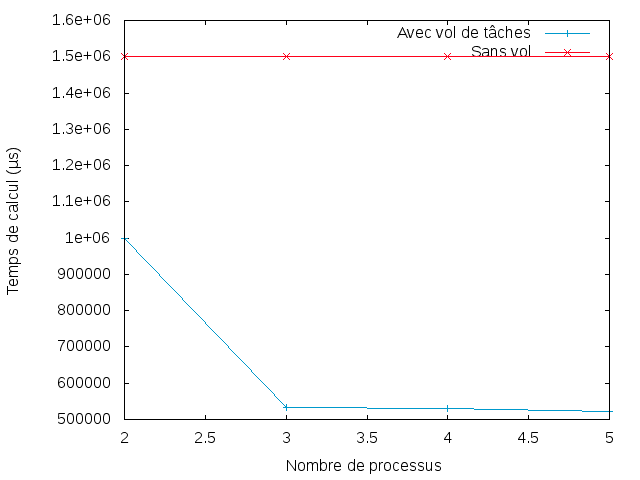
\includegraphics[width=0.8\textwidth]{vol_lin_lin}
\caption{Restes lin}
\label{vol_lin_lin}
\end{figure}
On peut voir sur la figure \ref{comp_chinois_vol} que le vol de travail avec une distribution linéaire est plus intéressant que d'utiliser les restes chinois.
\begin{figure}[H]
\centering
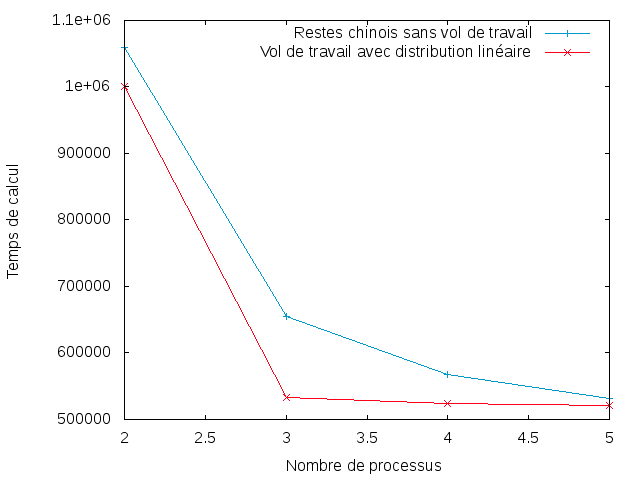
\includegraphics[width=0.8\textwidth]{comp_chinois_vol.png}
\caption{Le vol de tâche permet d'être plus rapide qu'une distribution statique (presque) idéale.}
\label{comp_chinois_vol}
\end{figure}

Enfin, il s'avère que faire du vol de tâches sur une distribution statique idéale n'apporte pas grand chose, comme l'exprime les figures \ref{vol_chinois_lin} et \ref{vol_chinois_chinois} .
\begin{figure}[H]
\centering
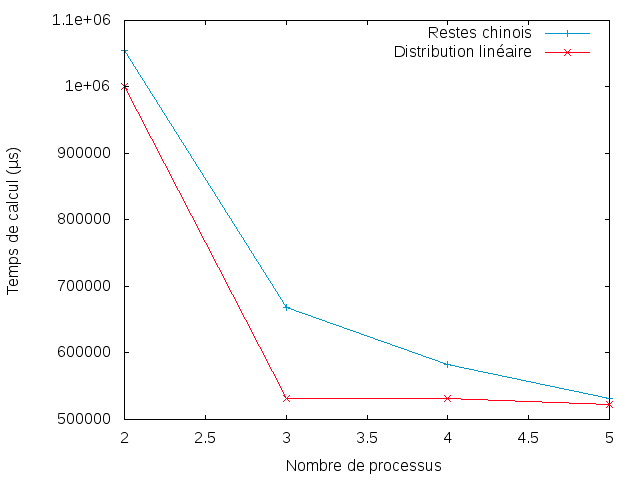
\includegraphics[width=0.8\textwidth]{vol_chinois_lin.png}
\caption{Avec vol de tâche.}
\label{vol_chinois_lin}
\end{figure}

\begin{figure}[H]
\centering
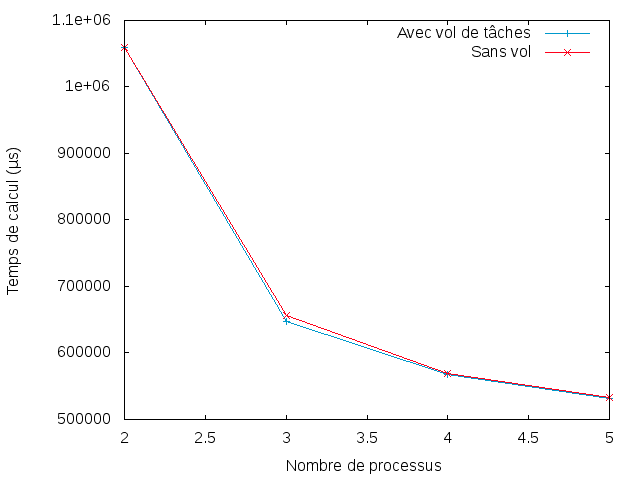
\includegraphics[width=0.8\textwidth]{vol_chinois_chinois}
\caption{Restes chinois}
\label{vol_chinois_chinois}
\end{figure}

